\documentclass[12pt,a4paper,openany,oneside]{book}
\nocite{*}


\usepackage[italian]{babel}
\usepackage[numbers]{natbib}
\usepackage{url}
\usepackage[hidelinks]{hyperref}
\usepackage{wrapfig}
%\usepackage[latin1]{inputenc} %Windows
\usepackage[utf8]{inputenc} %Linux
%\usepackage[applemac]{inputenc} %Mac
\usepackage{graphicx}
\usepackage{float}
\usepackage[font=small,labelfont=bf,tableposition=top]{caption}
 
\usepackage{listings}
\usepackage{xcolor} % Optional: for coloring code
\definecolor{amber}{RGB}{255,191,00}

  \usepackage{courier}
 \lstset{
         language=C++,
         basicstyle=\footnotesize\ttfamily,
         numbers=left,           
         numberstyle=\tiny,       
         numbersep=5pt,        
         tabsize=5,                 
         extendedchars=true,         
         breaklines=true,
         keywordstyle=\textbf,           
         stringstyle=\color{black}\ttfamily,
         showspaces=false,       
         showtabs=false,           
         xleftmargin=17pt,
         framexleftmargin=17pt,
         framexrightmargin=5pt,
         framexbottommargin=4pt,
         showstringspaces=false          
 }
 \linespread{1.23456789} % equivalente a 1.5 linee
 \addto\captionsitalian{%
 	\renewcommand{\lstlistingname}{Codice}}

\setcounter{tocdepth}{3} % fa apparire le subsubsection nell'indice
\setcounter{secnumdepth}{3} % e le numera


\usepackage{amsmath}


\usepackage{framed}

\begin{document}

%Inserisce qui il frontespizio
\begin{titlepage}
\centering 

\includegraphics[width=2.434cm,height=2.565cm]{Images/university_logo.png}

\bigskip

{\Large \textbf{UNIVERSIT\`A DEGLI STUDI DI CATANIA}}

{\scshape
\large
Dipartimento di Matematica e Informatica
}

{\scshape
\normalsize
Corso di Laurea Triennale in Informatica
}

\bigskip


\hrule


\bigskip


\bigskip


\bigskip


\bigskip

{\itshape
\large
Marco Spampinato
\par}


\bigskip


\bigskip


\bigskip


\bigskip

{\centering
\Large
Sviluppo e progettazione di un framework per il Digital Twin multi-agente distribuito
\par}


\bigskip


\bigskip


\bigskip


\bigskip


\bigskip


\bigskip


\begin{minipage}[b]{8 cm}
\hrule

\bigskip

{\centering\scshape 
Relazione Progetto Finale
\par}


\bigskip

\hrule
\end{minipage}
\bigskip


\bigskip


\bigskip


\bigskip


\bigskip


\bigskip


\bigskip


\bigskip


\bigskip


\bigskip


\bigskip

{\raggedleft
{\scshape Relatore} \\ {\itshape Prof. Federico Fausto Santoro}  \\
{\scshape Correlatore} \\ {\itshape Dott. Alessio Tudisco}
\par}


\bigskip


\bigskip


\bigskip


\bigskip

\hrule

\bigskip

{\centering
Anno Accademico 2024 - 2025
\par}
\end{titlepage}
 %<- richiama il file "parts/titlepage.tex" che contiene il frontespizio

\bibliographystyle{unsrtnat}
\title{Sviluppo e progettazione di un framework per il Digital Twin multi-agente distribuito}
\author{Marco Spampinato}

%Inserisce qui l'abstract
\chapter*{Abstract} %l'asterisco dopo chapter serve per visualizzare il capitolo come "non numerato"

I Digital Twin sono una tecnologia emergente e trasversale, il loro impiego spazia dalla manutenzione predittiva di macchine industriali, alla gestione di flotte di agenti mobili autonomi. In molti contesti applicativi, la gestione e coordinazione di molteplici e differenti agenti presenta una sfida non banale. Questa tesi propone la implementazione di un framework per la realizzazione di complessi sistemi multi-agente di Digital Twin e distribuita, fondato sullo stato dell'arte presentato da carissimi colleghi e professori nella pubblicazione \textit{Advancing Robotic Systems with Distributed Multi-Agent Digital Twins: A Scalable and Adaptive Framework} \cite{Russo2025}.



% La crescente disponibilità nel mercato odierno di soluzioni robotiche già pronte, \textit{off-the-shelf},
%  destinate al pubblico e sempre più performanti,
% ha reso accessibile lo sviluppo e la condivisione di progetti relativi alla robotica 
% come mai prima d'ora.
% 
% La robotica ripercorre un percorso già visto nell'ambito dello sviluppo di videogiochi,
% con il primo framework nel 2005 per il game development con licenza gratuita.
% 
% Il presente lavoro accoglie le ultime novità nel game development e nella robotica accessibile,
% attraverso la progettazione di un videogioco che impiega la tecnologia del Digital Twin, con l'obiettivo
% di esplorare nuove forme di interazione tra mondo reale e virtuale, promuovendo al contempo un'esperienza divertente e innovativa.
% A tale scopo, mediante il potente ecosistema di sviluppo offerto da \textit{Espressif} per l'Alvik,
% la libreria \textit{enet} per le comunicazioni, e il versatile motore di gioco \textit{Godot}, 
% è stato prodotto un videogioco multi giocatore, dove quattro player possono sfidarsi
% all'interno di una \textit{arena virtuale e fisica}.
% 
% Nel videogioco, ogni player comanda un carro, tale carro è intepretato nel mondo reale da un
% Alvik, il quale condividerà con il suo gemello virtuale informazioni sull'ambiente circostante. \\
% Ogni carro è dotato di cannone laser e tre palloncini, l'obiettivo è quello di far scoppiare i
% palloncini degli avversari: vince l'ultimo giocatore in gioco dotato di palloncini.
% 

%Genera l'indice
\tableofcontents

\chapter{Introduzione}

In tempi recenti, il Digital Twin si è affermato come una delle tecnologie più trasformative dell'Industria 4.0.
\noindent Inizialmente concepito in ambito aerospaziale allo scopo di monitorare lo stato dei veicoli spaziali, il gemello digitale è diventato rapidamente una tecnologia trasversale in tutti i campi aperti al progresso tecnologico. Chiave del suo successo è la fusione di modelli matematici e dati reali, il gemello digitale permette la realizzazione di strumenti che spaziano dalla predizione di guasti alla coordinazione di complessi sistemi e processi.

In contemporanea alla sua diffusione in ambito industriale, al fine di monitorare lo stato degli impianti e macchine di produzione, si è assistita a una rapida crescita dell'interesse accademico alla tecnologia, tale da scaturire una rapida proliferazione di interessanti articoli scientifici estesi non più solo in campi industriali, ma anche in settore primario e servizi.

Diverse ricerche sui digital twin hanno esplorato soluzioni nell'ambito delle \textit{smart cities} \cite{dt_smart_cities} e l'integrazione di gemelli digitali con dispositivi IoT nella pianificazione urbana; in agricoltura sono state studiate applicazioni per il monitoraggio delle colture \cite{dt_agricolture}; nelle \textit{smart grids} \cite{smartgerudo} nel contesto della distribuzione energetica in combinazione all'uso di intelligenza artificiale. Come è facile evincere, la ricerca si propaga nella direzione di sistemi sempre complessi di gemelli digitali.

L'integrazione di gemelli digitali in sistemi multi-agente è di chiave importanza in molti dei contesti citati: nelle smart cities, veicoli a guida autonoma possono coordinare percorsi al fine di ridurre congestioni; in agricoltura gemelli digitali di robot possono collaborare nel campionamento delle colture al fine di individuare eventuali fitopatie nelle piante.

Tali sistemi multi-agenti richiedono opportune infrastrutture software, scalabili e robuste, al fine di supportare cooperazioni su larga scala.


Il presente lavoro di tesi si occuperà di sviluppare una implementazione di un framework per la realizzazione di sistemi di gemelli digitali multi-agente distribuito, fondando la sua base teorica sull'architettura presentata dall'articolo scientifico \textit{Advancing Robotic Systems with Distributed Multi-Agent Digital Twins: A Scalable and Adaptive Framework} \cite{Russo2025}.

Dai principi e obiettivi fissati nella pubblicazione di riferimento, è stata realizata una suite di software in grado di collegare dispositivi embedded e simulazione nel motore \textbf{Godot Engine}, implementare gemelli digitali con questo collegamento, e orchestrare un ambiente virtuale condiviso tramite le API per il networking di Godot stesso.

\bigbreak 

%I Digital Twin (repliche virtuali di sistemi fisici) sono diventati strumenti fondamentali nella robotica, nell'industria 4.0, nella sanità e nelle smart city. Permettono di simulare scenari, prevedere guasti e ottimizzare le prestazioni in tempo reale senza rischi, riducendo costi e tempi di fermo. L'integrazione con l'Intelligenza Artificiale (IA) sta portando a sistemi sempre più autonomi e intelligent\section{Caso di studio}
 

\subsubsection*{Struttura della tesi}
Nei successivi capitoli verranno trattati i seguenti argomenti:
\begin{itemize}
  \item Il \textbf{Capitolo 2} descrive il modello del DMDTE.

  \item Il \textbf{Capitolo 3} introduce le tecnologie software e hardware utilizzate.
  \item Il \textbf{Capitolo 4} descrive nel dettaglio l'implementazione di DMDTE, descrivendone architettura, implementazione e uso.
  \item Il \textbf{Capitolo 5} discute delle varie sperimentazioni eseguite con il framework. 
\end{itemize} %<- richiama il file "parts/capitolo1.tex" che contiene il primo capitolo
\chapter{DMDTE}
%\section{Cosa è un Digital Twin}
%Un \textit{digital twin} - in italiano \textit{gemello digitale} - è la copia digitale di un oggetto fisico e reale, sia questo oggetto ancora nella fase di progettazione, fase di prototipazione, fase di validazione, o in fase di uso operativo.
%\medbreak
%\
%Affinché un digital twin si possa considerare tale, quindi non più strettamente coincidere con la simulazione di un sistema o model, il gemello digitale deve essere in qualche \textit{relazione con l'ambiente reale}.
%\medbreak
%Definiamo allora come \textit{real twin} la controparte fisica e reale del \textit{digital twin}, \textit{digital model} un model totalmente digitale della controparte fisica, e come \textit{thread} - \textit{filo} in italiano - il flusso di dati bidirezionale tra i due gemelli.
%\medbreak
%Distinguiamo anche l'ambiente operativo di real twin e digital model:
%\begin{itemize}
%	\item Il \textbf{real twin} ha come ambiente di lavoro il \textbf{mondo reale}, pertanto percepisce questo per mezzo di \textit{sensori}, e a sua volta interagisce su di esso per mezzo di \textit{attuatori}.
%	\item Il \textbf{digital model} ha come ambiente di lavoro un \textbf{mondo virtuale}, il quale deve essere quanto più fedele possibile nel rappresentare la sua controparte reale, tuttavia non precludendo la possibilità di possedere \textit{informazioni aggiuntive}, come oggetti puramente virtuali, o anche semplificazioni di modelli cinematici e dinamici; il digital twin interagisce con l'ambiente virtuale mediante gli strumenti messi a disposizione dal software in cui questo è sviluppato, i quali potrebbero anche essere a loro volta digital twin di sensori o attuatori reali; infine, in quanto questo sia un mondo digitale, non vi è incertezza d'informazione, pertanto è possibile interrogare il sistema mondo e ottenere informazioni esatte su di esso e le entità che lo popolano.
%\end{itemize}
%
%Allora, possiamo definire il \textbf{digital twin} quando vi è uno scambio di dati, un \textit{thread} o \textit{filo} tra le due entità, quindi un digital twin è una entità che \textbf{interagisce con} e \textbf{percepisce} entrambi i mondi, \textbf{reale} e \textbf{digitiale}.
%
%\subsection{Livelli di integrazione}
%Le definizioni date fino ad ora, sono basate sul lavoro svolto da Werner Kritzinger et al. \cite{KRITZINGER20181016}, il quale articolo si presenta come una analisi categorica della letteratura scientifica sui digital twin fino all'anno 2018, formalizzando il concetto di digital twin secondo le sue relazioni con l'ambiente reale.
%
%In particolare, tale lavoro si propone come punto di incontro tra le varie definizioni di digital twin, andando ad individuare tre sottocategorie di gemelli digitali come mostrato in Figura. \ref{fig:dt_data_integration}, differenziandole in base al flusso di dati scambiati tra i due gemelli, in particolare vengono suddivisi in \textit{digital model}, \textit{digital shadow} e \textit{digital twin}.
%
%\begin{itemize}
%	\item Un \textbf{digital model} è un model digitale di un oggetto, esso può essere messo in relazione con l'ambiente reale, e quindi il gemello reale, tuttavia ciò non è necessario o richiesto, lo scambio è manuale.
%	\item Un \textbf{digital shadow} è un digital model che riceve dati dall'ambiente esterno per mezzo del gemello reale, tuttavia non è necessario che questo interagisca con l'ambiente reale.
%	\item Un \textbf{digital twin} è quindi un digital shadow che scambia attivamente dati con l'ambiente reale per mezzo del gemello reale, pertanto interagisce attivamente con l'ambiente reale e risponde ad esso.
%\end{itemize}
%
%Come già accennato, è ruolo del \textit{thread} mettere in comunicazione il gemello reale e il gemello digitale. 
%\begin{figure}[htbp]
%  \centering
%  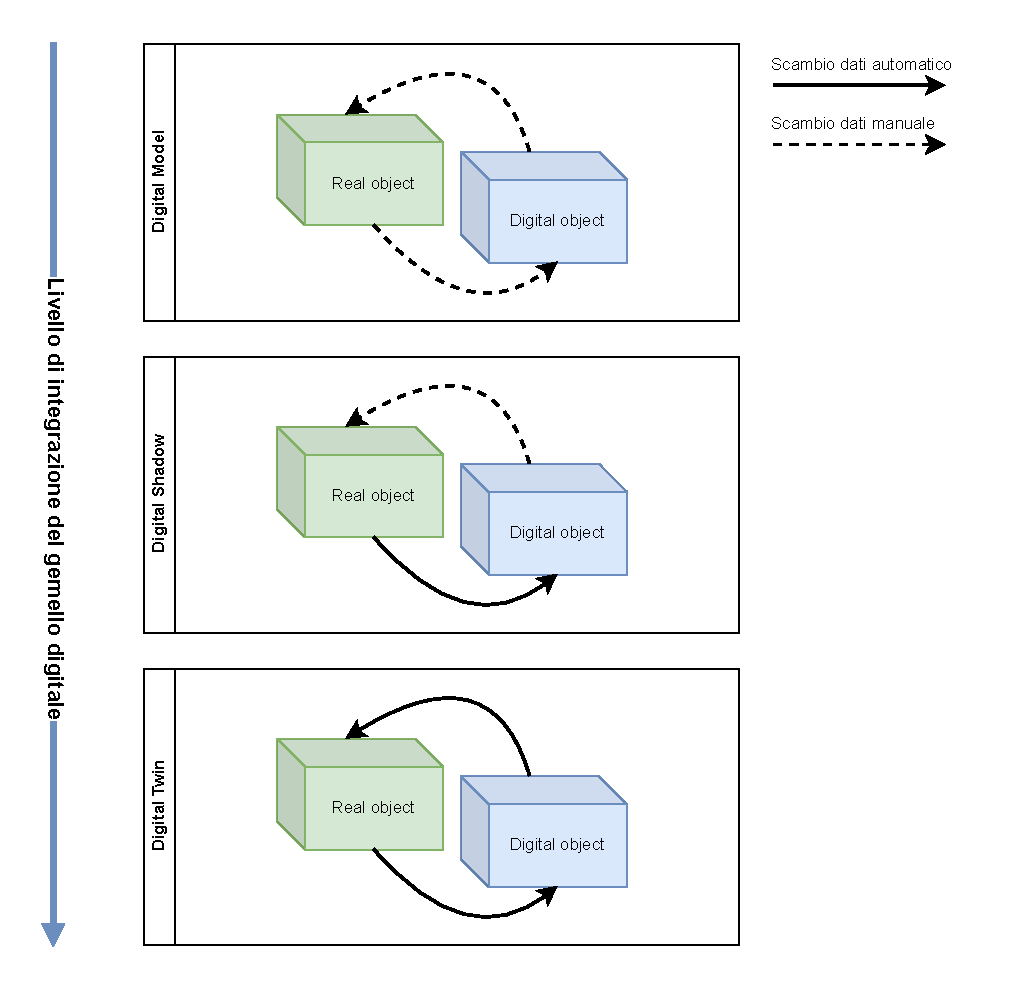
\includegraphics[width=1.0\textwidth, page=1]{Images/cristo.pdf}
%  \caption{Livelli di integrazione dati nei digital twin.}
%  \label{fig:dt_data_integration}
%\end{figure}
%
%
%\subsection{Origine}
%Non è possibile andare ad individuare una origine ben precisa dell'idea del digital twin, in quanto si può considerare una convergenza di idee, infatti noi umani studiamo ambiente e oggetti circostanti, creandone una rappresentazione mentale per mezzo dei nostri organi sensoriali, processi cognitivi e conoscenza, con tale rappresentazione dunque riconosciamo ambienti per navigare con più sicurezza, riconosciamo e usiamo oggetti con padronza: pertanto trasporre questo nostro processo intrinseco in ambito computazionale non è che una conseguenza del fatto che questo processo, naturale e trasparente per noi, sia una idea vincente da applicare per sistemi artificiali più intelligenti, sicuri e affidabili.
%\medbreak
%Una prima formalizzazione in letteratura viene da uno studio sul \textit{Product lifecycle management} PLM - in italiano \textit{gestione del ciclo di vita di un prodotto} - nel 2005 da Grieves \cite{grieves2005}, nel suo studio sul ciclo di vita di un prodotto - ideazione, produzione, operatività e smaltimento - considera fondamentale l'informazione, introduce pertanto il concetto di \textbf{Mirrored Space Models}, un model che consiste dei tre elementi che caratterizzano  anche l'idea moderna del digital twin: oggetto fisico, model virtuale e scambio di dati tra loro.
%\medbreak
%
%La nascita del termine vero e proprio di digital twin lo sì deve alla NASA in ambiente aerospaziale, in particolare in \textit{The digital twin paradigm for future NASA and U.S. air force vehicles (2012)} \cite{nasa2012} viene introdotto il digital twin come un complesso e ultra realistico model simulativo del veicolo reale, il quale usa i migliori modelli fisici disponibili, sia integrato con i sistemi e sensori del veicolo e sia esattamente speculare al veicolo stesso. L'obiettivo del digital twin secondo NASA è quello di salvaguardiare ulteriormente lo stato di salute del veicolo quando questo è in missione, fornendone un model digitare per il monitoraggio del veicolo, correzione degli errori, mitigazione danni e eventi non prevedibili etc. attività non immediatamente correggibili o prevedibili in fase di progettazione e produzione nonostante le migliori tecnologie, dunque per la seconda volta l'idea di base di digital twin si propone come strumento fondamentale per il ciclo di vita di un prodotto (il veicolo spaziale).
%\medbreak
%
%Dal 2016 in poi, con l'evoluzione tecnologica, l'introduzione massiva dell'Internet Of Things, la necessità dell'integrazione digitale nell'industria e nei prodotti di uso comune, la nascita dell'industria 4.0 con la sua esigenza di integrare il digitale con la produzione e il ciclo di vita dei prodotti, si osserva un significativo aumento della letteratura scientifica sugli studi relativi ai digital twin, correlata a una confusione generale del termine, specie nella sua relazione con \textit{digital model} e \textit{digital shadow}, come documentato da Werner Kritzinger et al. \cite{KRITZINGER20181016} e da \textit{Digital Twin: Origin to Future (2021)} \cite{origin2021}, cui definisce il digital twin come:
%
%\begin{quote}
%\textit{Un Digital Twin è un model o una simulazione digitale/virtuale, dinamica e capace di auto-evolversi, di un soggetto o oggetto reale (componente, macchina, processo, essere umano, ecc.), che rappresenta lo stato esatto del suo gemello fisico in ogni istante tramite lo scambio di dati in tempo reale e la conservazione dei dati storici. Non è solo il Digital Twin a imitare il suo gemello fisico: anche qualsiasi variazione nel Digital Twin viene imitata dal gemello fisico.}
%\end{quote}
%
%\pagebreak
\parbox{1.0\textwidth}{
	\textbf{Distributed Multi Agent Digital Twin Environment} (DMDTE) è una \textit{architettura} per la progettazione di complessi sistemi multi-agente Digital Twin.
}
\medskip

Al fine di comprendere la sua implementazione, è necessario spiegare il suo modello generale.

Consideriamo, in ordine, un modello più semplice singola a istanza e singolo gemello digitale al fine di chiarere i concetti di base, successivamente viene introdotto il modello più generale distribuito e multi istanza.
\pagebreak
\begin{figure}[ht]
  \centering
	\includegraphics[page=2, width=1.0\textwidth]{Images/cristo.pdf}
	\caption{Modello singolo agente: in basso l'ambiente reale e le sue entità, in alto ambiente virtuale con le sue entità, tra esse digital twin di entità reali.}
  \label{fig:dmdte-single-instance}
\end{figure}
\section{Modello singolo agente}
\parbox{1.0\textwidth}{
	Il modello singolo agente fornisce un ottimo punto di partenza per la descrizione di un sistema digital twin ad agenti, possiamo trovare una sua rappresentazione grafica nella \autoref{fig:dmdte-single-instance}, la quale illustra un semplice sistema digital twin a singolo agente.
	}
\medbreak


Bisogna distinguere due ambienti: 
l'\textbf{ambiente reale}, posto nella parte inferiore della figura, contiene le entità reali del mondo reale, nel caso di esempio un peluche e un robot; l'\textbf{ambiente virtuale}, posto nella parte superiore della figura, è una copia virtuale dell'ambiente reale, del quale ne emula topologia e proprietà fisica, ed è popolato da \textit{digital twin} e \textit{virtual agent}.

L'\textbf{ambiente virtuale} è interamente simulato da un software, nella implementazione presentata \textit{Godot}, in esso vi possiamo trovare:
\begin{itemize}
	\item Il \textbf{digital twin} di un agente robotico reale in esempio un Alvik.
	\item Il \textbf{digital twin} di un oggetto o ostacolo reale, in esempio un peluche di \textit{capybara}.
	\item \textbf{Agenti virtuali} e \textbf{ostacoli virtuali}, in esempio un agente robotico virtuale, un ostacolo a forma di cono stradale e un ostacolo a forma di parallelepipedo.
\end{itemize}

Come si può notare dalla figura, gli oggetti reali hanno una corrispondenza digitale: il \textit{digital twin}. Oggetti statici come il peluche di capybara possono essere rappresentati staticamente nel mondo virtuale con approssimate geometrie, sufficienti a rappresentarne una presenza nello spazio come ostacolo.
\medskip

Gli \textbf{agenti robotici} o dinamici, analogamente agli ostacoli, possiedono un \textit{digital twin}, dotato di uno flusso bidirezionale e automatico di informazioni per mezzo di un \textit{collegamento} fra il \textit{real twin} e \textit{digital twin} \cite{KRITZINGER20181016}. Nel contesto del DMDTE il real agent deve possedere una unità di calcolo sufficiente per eseguire la \textbf{Real Agent Interface}, una API che esponga le funzionalità e lo stato dell'agente stesso.
\medbreak

Il \textit{Real Agent Interface} comunica per mezzo del \textbf{Digital Twin Protocol}, in breve DTP, con la sua controparte digitale. Il DTP è un protocollo di comunicazione realizzato per DMDTE, il suo scopo è quello di permettere la sincronizzazione di stato tra agente reale e gemello digitale e l'invocazione di metodi per mezzo di \textit{chiamate a procedura remota}.
Nel contesto di DTP, identifichiamo come peer DTP un gemello reale o virtuale, e come DTP host l'applicazione che ospita gemelli digitali e permette la loro comunicazione con il loro reale.
\medbreak

Il \textit{digital twin} dell'agente robotico, infine, è una entità composta da due oggetti: il \textit{model} dell'agente robotico, in grado di interagire con l'ambiente virtuale, e il \textit{ghost}. Il ghost è sincronizzato in tempo reale per mezzo di DTP con l'agente reale, tuttavia come un fantasma, non è in grado di interagire con l'ambiente virtuale. Il model è potenzialmente in grado di interagire con l'ambiente virtuale, deve essere dotato di un modello tridimensionale, dinamiche fisiche, e deve interagire con l'ambiente virtuale in modi quanto più simili a come il gemello reale interagisce con l'ambiente reale. 
\medbreak

Ghost e model sono sempre tenuti in \textit{stretta vicinanza} e corrispondenza di posa, inoltre le simulazioni fisiche avvenute nel model digitale, successivamente alla loro esecuzione, si ripercuotono nel gemello reale tramite DTP, il cui a sua volta risponderà di conseguenza riportando il suo stato successivo al \textit{ghost}, andando così a costruire un sistema di feedback automatico.
\medbreak

Assegnando dei \textbf{controller} al model, ovvero programmi o script che definiscono uno specifico comportamento e controllo definiti dal programmatore in Godot, è possibile specificare un comportamento ben preciso per il digital twin: è allora possibile definire un controller che segua un determinato percorso, sia questo definito da una logica dettata da sensori di prossimità, line follower o da un \textit{navigation agent} di Godot, oppure permettere a un utente umano il controllo del robot: controllando il \textit{model}, viene a sua volta coinvolto il \textit{real twin}, e di conseguenza aggiornato il \textit{ghost}, creando un ciclo di feedback automatico; pertanto si identifica il sistema \textit{ghost/model} come gemello digitale.
\medbreak

Infine è possibile anche definire \textbf{agenti completamente virtuali}, ovvero entità dinamiche del mondo virtuale che non hanno corrispondenza reale, controllabili con gli stessi \textit{controller} definiti per il \textit{digital twin/model}, tali agenti possono essere utili per effettuare pure simulazioni, esplorare ambienti, aggiungere ostacoli dinamici, oppure rappresentare all'interno dell'ambiente virtuale entità reali la quale tuttavia si ha un alto grado di incertezza relativa sul loro stato, come per esempio entità catturate da un sistema di computer vision.
\medbreak


\begin{figure}[t]
  \centering
	\includegraphics[page=3, width=1.0\textwidth]{Images/cristo.pdf}
  %\includegraphics[width=1.0\textwidth]{Images/distributed-multi-agent.drawio.pdf}
  \caption{Modello del sistema multi agente e distribuito}
  \label{fig:dmdte}
\end{figure}
\section{Modello multi agente distribuito}
Definito il modello a singolo agente semplice, consideriamo lo scenario in cui più agenti robotici e più istanze di mondi virtuali debbano coesistere e coordinarsi tra loro.
\medbreak

Senza perdere di generalità, consideriamo il caso di due agenti digital twin e tre istanze di ambiente virtuale, tale architettura è esemplificata dalla Figura \ref{fig:dmdte}.
\medbreak

Come mostrato in figura, ognuno degli agenti robotici è collegato per mezzo di DTP a una istanza esclusiva di Godot, una terza istanza di Godot funge da osservatore: ogni istanza è in comunicazione con le altre per mezzo della \textbf{MultiplayerAPI}, un insieme di strumenti e API che permettono la creazione di un ambiente virtuale replicato tra istanze di rete integrato in Godot, la quale in modo trasparente al programmatore si occupa della sincronizzazione dello stato delle entità presenti nella scena, dell'ambiente virtuale e la gestione di eventuali comunicazioni per mezzo di \textit{chiamata a procedura remota}. Nel contesto della \textit{MultiplayerAPI}, la singola istanza di Godot prende il nome di \textbf{multiplayer peer}. Un peer multiplayer può anche essere un \textit{DTP host} e ospitare più istanze di \textit{digital twin}, in tal caso identifichiamo come \textit{autorità} l'istanza di \textit{multiplayer peer} che ospita un determinato \textit{digital twin} e il suo DTP peer; una istanza può non ospitare alcun gemello virtuale o non essere DTP host e comportarsi da semplice osservatore.
\medbreak

Con questo modello, le istanze di ambiente virtuale e agenti digitali sono replicati e sincronizzati, permettendo una integrazione trasparente di unità di calcolo eterogenee in grado di collaborare tra loro per coordinare gli agenti.
\medbreak

Gemelli digitali anche di diverse istanze allora possono collaborare tra loro per compiere task in modo coordinato.
 %<- richiama il file "parts/capitolo2.tex" che contiene il primo capitolo
\chapter{Tecnologie utilizzate}
Nella produzione del progetto di tesi sono stati utilizzati
una eterogenea varietà di soluzioni terzi, in breve:
\begin{itemize}
	\item \textbf{Godot Engine} come ambiente di simulazione tridimensionale. 
	\item La libreria di rete \textbf{ENet} .
	\item \textbf{Arduino Alvik} come robot mobile. 
% \item \textbf{Blender} per la realizzazione di assets personalizzati.  
\end{itemize}

Sono stati inoltre utilizzati i seguenti linguaggi di programmazione:
\begin{itemize}
	\item \textbf{C++} per la realizzazione del software eseguito dall'\textbf{Arduino Alvik}.
	\item \textbf{GDScript}, il linguaggio di scripting di Godot, per la realizzazione della logica all'interno del motore di gioco.
\end{itemize}

\pagebreak
\section{Godot Engine}
\textbf{Godot} \cite{GodotEngine} è un motore di gioco multi piattaforma gratuito e open source,
rilasciato su licenza MIT, in sviluppo dal 2014; leggero e completo, permette la creazione di simulazioni e giochi bidimensionali e tridimensionali tramite composizione di nodi che prendono nome di \textit{scene tree} o albero di scena. \\
Programmi scritti dallo sviluppatore chiamati \textit{script} e associati ai nodi della scena rendono dinamica e interattiva quest'ultima.
\medbreak

Godot vanta di una solida componente di \textit{rendering} in grado di supportare nuovo e vecchio hardware, non di meno piattaforme mobile come Android e iOS, con solido supporto  per le popolari API grafiche come Vulkan e DirectX 12 per il desktop, OpenGL ES per il mobile; è anche possibile eseguire software Godot in modalità \textit{headless}, ovvero senza rendering, il quale non è necessario qualora si volesse eseguire una istanza di server.

\medbreak
Nell'ambito delle simulazioni fisiche, Godot vanta di un suo motore fisico interno completo di simulazioni cinematiche e dinamiche, corpi rigidi e \textit{soft-bodies}, vincoli fisici o \textit{constraints}, giunti e motori, simulazione di veicoli e sospensioni; inoltre, data la sua natura modulabile, è possibile implementare o scegliere una implementazione terza della componente fisica, di particolare nota è la disponibilità di \textbf{Jolt} \cite{JoltPhysics}, un motore fisico annoverato per le sue capacità e efficienza, ampliamente affermato nell'industria videoludica; seppure non utilizzato nella soluzione proposta, sì intende esplorare Jolt in applicazioni future.

Godot vanta di diverse componenti interessanti, tuttavia vengono approfondite in seguito solo quelle di particolare interesse ai fini del lavoro svolto.

\subsection{GDScript}
\textbf{GDScript} \cite{GodotGDScriptDocs} è un linguaggio di programmazione ad alto livello, orientato agli oggetti, imperativo e progressivamente tipizzato nonché il linguaggio di scripting ufficiale di Godot.
\medskip

Integrato all'interno di Godot, insieme agli strumenti di language server e debugging, ha una sintassi leggera simile a Python, dispone di tutti i tipi specifici necessari alla manipolazione degli oggetti di scena come tipi scalari interi e reali, vettoriali, matriciali, array, stringhe, dizionari e ulteriori oggetti complessi; non mancano anche moduli e librerie per la serializzazione, espressioni regolari, input, networking, storage, concorrenza e interfacce ai sistemi del motore di gioco.

Di particolare nota è la natura di GDScript come linguaggio interpretato, la quale condizione comporta una maggiore facilità d'uso e una più veloce iteratività, a discapito di performance inferiori rispetto un linguaggio compilato; tuttavia è possibile programmare Godot anche in linguaggi compilati come C++ e interagire con tali componenti in GDScript, così da delegare sistemi complessi o pesanti elaborazioni a codice più veloce, non rinunciando alla flessibilità di un linguaggio di scripting.

\subsection{Networking in Godot}
Godot permette due principali e diversi approcci \cite{GodotMultiplayerDocs} sul \textit{networking} o \textit{multiplayer}:
\begin{itemize}
	\item L'approccio \textbf{High-level} consiste nell'uso di strumenti di alto livello integrati in Godot per la realizzazione di un modello client-server autoritativo.
	\item Un approccio \textbf{Low-level}, dove è responsabilità dello sviluppatore gestire connessione, protocollo di comunicazione tra client, spawn e sincronizzazione; Godot integra diversi protocolli e librerie, in particolare UDP, TCP, ENet, WebSocket, WebRTC e HTTP.
	\item Un terzo approccio, \textbf{mid-level}, consiste nella implementazione da parte dello sviluppatore delle interfacce richieste dall'\textit{high-level networking}, al fine di usarne gli strumenti con protocolli o caratteristiche differenti.
\end{itemize}
\medbreak

L'approccio di alto livello si basa su una particolare implementazione di un oggetto coordinatore chiamato \textit{MultiplayerScene}, di cui Godot fornisce implementazione per i medesimi protocolli e librerie di basso livello disponibili; è un approccio che prevede autorità al fine di compiere determinate azioni, l'autorità è del server e può essere ceduta ai client.
\smallbreak
Strumenti fondamentali offerti da questo approccio gestito sono:
\begin{itemize}
	\item Le \textit{chiamate a procedura remota} o \textbf{RPC}, che permettono di richiamare su di un secondo peer una determinata funzione.
	\item Il \textbf{MultiplayerSpawner}, un oggetto che si occupa di sincronizzare lo spawn di entità dalla istanza server ai client.
	\item Il \textbf{MultiplayerSynchronizer}, un oggetto che si occupa di sincronizzare stato da una istanza autorevole alle altre.
\end{itemize}

Entrambi gli strumenti di basso livello e di alto livello sono stati utilizzati nella proposta implementazione di DMDTE e saranno successivamente richiamati, descrivendone eventuali sfide affrontate e criticità.

% Nell'implementazione prodotta del DMDTE, gli strumenti offerti da Godot per l'approccio \textit{low-level} sono stati utilizzati per realizzare il \textit{Digital Twin Protocol}, il protocollo di comunicazione implementato per legare \textit{real twin} alle corrispondenti istanze di \textit{digital twin} ospitate da una istanza di Godot, per mezzo della implementazione di ENet esposta





\section{ENet}
\textbf{ENet} \cite{ENetLibrary} è una libreria \textit{C} che fornisce una astrazione di alto livello
per comunicazione di rete orientate alla connessione, ma basata su UDP, 
offre opzionalmente trasmissione ordinata e affidabile di messaggi tra peer.
\medskip

Tali caratteristiche hanno reso ENet molto popolare nei software che richiedono comunicazioni real-time, 
in particolare nei videogiochi: ENet è ampliamente utilizzata per la realizzazione
delle componenti multiplayer, Godot stesso implementa interfacce di basso e alto livello
per il networking con ENet.
\medskip

È stato necessario realizzare un \textit{fork} di ENet\cite{enet_esp32} al fine di rendere compatibile la libreria con la piattaforma embedded utilizzata, tali modifiche sono documentate nel successivo capitolo.
%;
%scopo di rendere ENet compatibile con l'ambiente di sviluppo \textit{ESP-IDF},
%in quanto sì è rivelata limitata l'implementazione delle \textit{socket} e assente
%la presenza di alcune procedure di sistema \textit{UNIX}, in particolare \textit{epoll}.

\section{Arduino Alvik}
\begin{figure}[htbp]
  \centering
  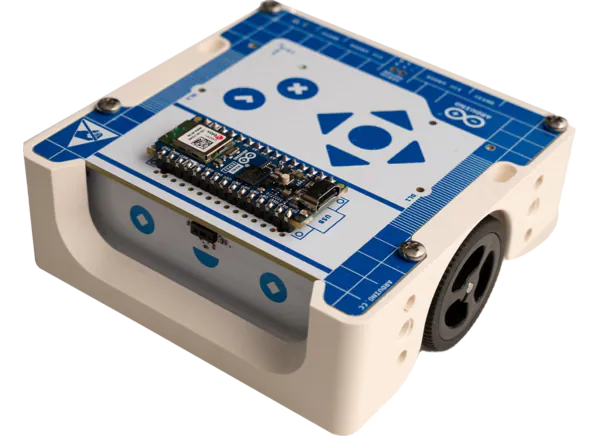
\includegraphics[width=0.6\textwidth]{Images/alvik}
  \caption{Arduino Alvik.}
  \label{fig:immagine}
\end{figure}
L'\textbf{Alvik} \cite{ArduinoAlvik} è una piattaforma robotica educativa e modulare sviluppata da \textit{Arduino},
progettato per introdurre studenti e utenti alle prime armi al mondo della robotica,
non sacrificando prestazioni e estendibilità.
\medskip

È dotato di due microcontrollori e una vasta gamma di sensori e attuatori. \\
Il microcontrollore principale è un \textit{Arduino Nano ESP32},
posizionato nella parte superiore e gestisce la logica di alto livello.
All'interno del corpo del robot, denominato \textit{carrier}, è invece integrato
un microcontrollore \textit{STM32F4}, responsabile del controllo dei sensori e attuatori. \\
L'architettura a doppio controllore permette una maggiore disponibilità di risorse per le applciazione degli utenti, i quali sono generalmente eseguiti dall'Arduino Nano.
\medskip

Il robot è dotato di un ampio set di sensori e attuatori che gli permettono di percepire l'ambiente circostante e interagire attivamente con esso.
\pagebreak
\begin{table}[h!]
\centering
\renewcommand{\arraystretch}{1.2}
\begin{tabular}{|p{4cm}|p{9cm}|}
\hline
\textbf{Microcontrollore principale} &
Arduino Nano ESP32: 
\begin{itemize}
  \item 8 MB RAM
  \item u-blox® NORA-W106 (ESP32-S3)
  \item Processore fino a 240 MHz
  \item ROM 384 kB + SRAM 512 kB
  \item 16 MB di memoria FLASH esterna
\end{itemize} \\ \hline

\textbf{Secondo microcontrollore} & STM32 Arm® Cortex®-M4 32 bit \\ \hline

\textbf{Alimentazione} & 
Nano ESP32 USB-C® con batteria Li-Ion 18650 ricaricabile e sostituibile (inclusa) \\ \hline

\textbf{Programmazione} & 
MicroPython, Arduino e programmazione a blocchi \\ \hline

\textbf{Connettività} & 
Wi-Fi®, Bluetooth® Low Energy \\ \hline

\textbf{Sensori e input} &
	Time of Flight Distance Sensor (fino a 350 cm),
	RGB Color Sensor,
	Giroscopio–accelerometro a 6 assi,
	Array line follower (x3),
	Pulsanti tattili (x7),
\\ \hline

\textbf{LED e motori} &
	2 LED RGB,
	Motori 6V – velocità a vuoto 96 rpm, corrente a vuoto 70 mA,
\\ \hline

\textbf{Estensioni} &
Connettori LEGO® Technic™ (x4),
Connettori a vite M3 (x8),
Servo motore,
I2C Grove,
I2C Qwiic,  \\ \hline
\end{tabular}
\caption{Specifiche tecniche del robot \textit{Alvik}.}
\label{tab:alvik-specs}
\end{table}

\subsection{Ambiente di sviluppo}
L'ambiente di sviluppo dell'\textit{Alvik} è \textbf{ESP-IDF}, il kit ufficiale di \textit{EspressIf} per i microcontrollori \textbf{ESP32},
a sua volta basato sul sistema operativo in tempo reale \textit{FreeRTOS}.

In tale ambiente sono disponibili una vasta e completa gamma di procedurre per la gestione di thread,
concorrenza, I/O e memoria proprie di \textit{FreeRTOS} e di \textit{ESP-IDF};
una implementazione della libreria standard \textit{C} e della \textit{STL} di \textit{C++};
varie implementazioni delle più importanti librerie usate nei sistemi \textit{UNIX} 
come \textit{pthread}, e di grandissima importanza, i \textit{Berkeley sockets}.
\medskip

Tale ricchezza ha permesso lo sviluppo di codice di alto livello \textit{portatile}, in grado
di essere facilmente utilizzato in altre piattaforme.
\medskip

Inoltre, la piattaforma \textit{Arduino}, fornisce una ulteriore astrazione a complesse operazioni,
come la configurazione di avvio del microcontrollore e la gestione del \textit{WiFi}.
\medskip

Specifica dell'\textit{Alvik} invece è la libreria per il controllo del \textit{carrier},
tale che fornisce una interfaccia a sensori e attuatori del robot, nonché servizi non banali
come odometria e stato della batteria.
\medskip



% \section{Blender}

%\begin{figure}[hb]
%  \centering
%  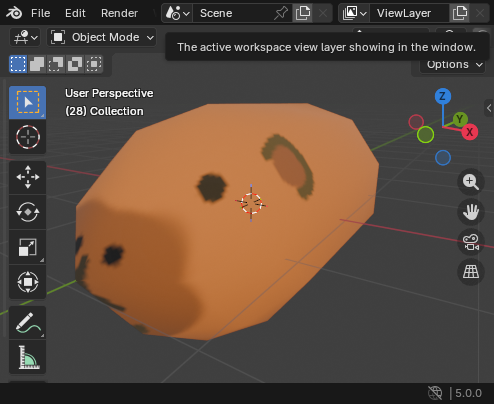
\includegraphics[width=0.5\textwidth]{Images/blender-screen.png}
%  \caption{Una schermata di Blender con assets prodotto.}
%  \label{fig:dmdte}
%\end{figure}


%Blender \cite{Blender} è un software open source e multipiattaforma per la modellazione, animazione e rendering 3D. \\
%È sviluppato e mantenuto dalla Blender Foundation ed è distribuito gratuitamente sotto licenza GPL. \\
%Il programma offre un set completo di strumenti per:
%\begin{itemize}
%	\item modellazione poligonale, NURBS e scultorea;
%	\item texturing e shading, con un potente motore di materiali basato su nodi;
%	\item animazione e rigging di personaggi;
%	\item simulazioni fisiche (fluido, fumo, tessuti, particelle);
%	\item rendering fotorealistico con i motori Cycles e Eevee;
%	\item video editing e compositing;
%	\item scripting in Python, utile per automatizzare o integrare funzionalità personalizzate.
%\end{itemize}	
%
%Grazie alla sua natura open source e all’ampia comunità di sviluppatori, Blender è oggi considerato uno degli strumenti più versatili e accessibili per la produzione 3D professionale e per l’insegnamento delle tecniche di computer grafica.
% %<- richiama il file "parts/capitolo3.tex" che contiene il primo capitolo
\chapter{Implementazione}
\begin{figure}[!htbp]
  \centering
  \includegraphics[width=\textwidth, page=4]{Images/cristo.pdf}
  \caption{Architettura DMDTE implementata.}
  \label{fig:architecture}
\end{figure}

In questo capitolo viene trattata l'implementazione del framework DMDTE, in ordine:
\begin{itemize}
	\item Specifiche e implementazione del \textbf{Digital Twin Protocol}.
	%\item Implementazione lato embedded della \textbf{Real Agent Interface}.
	\item Implementazione in Godot del \textbf{Digital Twin}.
	\item \textbf{Replicazione} e \textbf{sincronizzazione} della scena in Godot. 
\end{itemize}

Uno schema generale dell'architettura è illustrato dalla Figura \ref{fig:architecture}.
\pagebreak

\section{Digital Twin Protocol}
Il Digital Twin Protocol è un protocollo di scambio dati a livello utente, con architettura \textit{client-server}, non strettamente dipendente da uno specifico protocollo di trasporto, ma con i requisiti di \textit{affidabilità opzionale} e deve essere in grado di inviare pacchetti senza limitazione di dimensione ( quindi deve essere in grado di eseguire frammentazione ), ideato al fine di ottenere uno scambio dati leggero e veloce tra agenti robotici governati da microcontrollori embedded o dotati di computer di bordo, e istanze di Godot con i relativi gemelli digitali.

Di seguito entrambi gli agenti, real agent e digital twin, verranno chiamati \textit{DTP Peer}, inoltre va specificato che il Digital Twin Protocol si limita a definire scambi di dati e invocazione di messaggi, non definisce tipo di dati scambiati, ma solo la loro dimensione, infine sì considererà interfaccia di un DTP Peer l'insieme di metodi e proprietà esposte per mezzo del protocollo.
\smallbreak

Il protocollo definisce tre tipi di messaggi scambiati e relativi flussi e formati: \textbf{chiamata a procedura remota}, \textbf{messaggi di aggiornamento di stato} e \textbf{identificazione} tipo agente.


\begin{figure}[!hp]
  \centering
  \includegraphics[width=0.7\textwidth, page=6]{Images/cristo.pdf}
  \caption{Messaggio generico.}
  \label{fig:dtp-message-generic}
\end{figure}

I singoli messaggi hanno un formato base generico e binario: come mostrato in figura Figura \ref{fig:dtp-message-generic}, il primo byte del messaggio discrimina il tipo di messaggio inviato dal DTP Peer e assume valori tra \verb|0| e \verb|2|.

\subsection*{Chiamate a procedura remota}

I messaggi RPC o \textit{chiamate a procedura remota} hanno lo scopo di invocare determinate azioni o \textit{metodi} nel DTP Peer destinatario e sono in grado di trasportare argomenti e dati, come in Figura \ref{fig:dtp-message-rpc} sono discriminate da un tipo di messaggio \verb|0|, inoltre sono dotati dei campi:

\begin{itemize}
	\item Il campo \textbf{indice metodo} identifica il metodo da richiamare nel DTP Peer destinatario. Il campo è di tipo \textit{uint8}.
	\item Il campo \textbf{dimensione data} indica la dimensione del campo data. Il campo è di tipo \textit{uint16}.
	\item In coda il campo \textbf{data}, la cui dimensione è specificato dal precedente. Il campo ha \textit{lunghezza variabile}.
\end{itemize} 

\begin{figure}[h!]
  \centering
  \includegraphics[width=0.7\textwidth, page=7]{Images/cristo.pdf}
  \caption{Formato di messaggio di chiamata a procedura remota.}
  \label{fig:dtp-message-rpc}
\end{figure}
\bigskip

Come si intuisce, il DTP Peer mittente deve conoscere quale metodo invocare e con quale dati, viceversa il DTP Peer ricevente deve essere in grado di accettare la richiesta ed eseguire il metodo specificato dall'indice; la serializzazione e deserializzazione degli argomenti è a carico dello sviluppatore.

Si noti che il flusso di dati è attivo, ovvero il DTP Peer mittente invia manualmente il pacchetto, inoltre è necessario che tale pacchetto sia inviato in modo \textbf{affidabile}, ovvero il protocollo di trasporto usato deve garantire la ricezione e deve garantire che i messaggii arrivino in maniera ordinata.

\pagebreak

\subsection*{Messaggi di aggiornamento di stato}
I messaggi di aggiornamento di stato o \textit{Update} hanno lo scopo di sincronizzare stato tra i DTP Peer, in tale contesto identifichiamo come \textit{proprietà} una variabile di stato del \textit{real agent} e del \textit{digital twin} il quale valore deve essere sincronizzato alla variazione, identificata da un indice numerica, una proprietà inoltre può anche essere di sola lettura o sola scrittura in modo alterno per i DTP Peer considerati, allora identifichiamo una \textit{ownership} della proprietà e come \textit{owener} il DTP Peer che ha autorità su questa: per esempio nel caso di un sistema robotico, l'odometria è un sistema del real agent, pertanto la posa ha come \textit{owner} il real agent, viceversa un identificativo numerico del digital twin da mostrare su un display del real agent è di autorità del \textit{digital twin}; ancora una volta le specifiche di serializzazione e deserializzazione non sono specificate nel protocollo, sono a cura dello sviluppatore.

\begin{figure}[h!]
  \centering
  \includegraphics[width=0.7\textwidth, page=8]{Images/cristo.pdf}
  \caption{Formato dei messaggi di aggiornamento di stato.}
  \label{fig:dtp-message-update}
\end{figure}
\bigskip

Lo schema del formato dei messaggi è esemplificato dalla Figura \ref{fig:dtp-message-update}, il tipo di messaggio ha come numero identificativo \verb|1|, distinguiamo allora la testa del messaggio contenente informazioni speficiche alla interpretazione del messaggio, e in coda le singole proprietà scambiate, nel dettaglio i singoli campi:

\begin{itemize}
	\item \textbf{Numero proprietà} indica il numero di proprietà contenute nel messaggio scambiato, è possibile definire fino a 256 proprietà. Il campo è di tipo \textit{uint8}.
	\item Per ogni proprietà scambiata, si ha:
	\begin{itemize}
		\item Un campo \textbf{indice} che identifica la proprietà. Il campo è di tipo \textit{uint8}.
		\item Un campo \textbf{dimensione} che indica la dimensione del campo data. Il campo è di tipo \textit{uint8}.
		\item In coda il campo \textbf{data}. Il campo ha lunghezza variabile compresa tra 0 e 255 byte.
	\end{itemize}
\end{itemize}

Il flusso di scambio questa volta è passivo, il DTP Peer che ha autorità sulla proprietà deve notificare l'altro DTP Peer dei cambiamenti, può inviare sia pacchetti con solo le proprietà variate, o pacchetti con tutte le proprietà che rappresentano il suo stato, inoltre non vi è requisito di affidabilità, tuttavia è altamente consigliato di inviare lo stato completo del dispositivo robotico in modo affidabile in modo periodico.
\medbreak

È intuibile che le proprietà di un DTP Peer non sono altro che stato, questo stato può variare a seconda dei sistemi dei rispettivi attori, tramite chiamata RPC o tramite risposta alla variazione di una terza proprietà.

\subsection*{Messaggio di identificazione}
Il messaggio di identificazione è un messaggio inviato alla avvenuta connessione, ha lo scopo di notificare al \textit{DTPHost} quale tipo di agente reale si stia connettendo, e quindi di creare l'appropriato gemello digitale.

Il suo formato è illustrato in \autoref{fig:dtp-identification}, contiene un solo parametro \textbf{identificazione}, una stringa di lunghezza variabile, la cui dimensione è la dimensione in byte del messaggi a meno di un byte.

\begin{figure}[h!]
  \centering
  \includegraphics[width=0.7\textwidth, page=13]{Images/cristo.pdf}
  \caption{Formato del messaggio di identificazione.}
  \label{fig:dtp-identification}
\end{figure}
\bigskip


\subsection{Implementazione di DTP}



Il Digital Twin Protocol  nel progetto di tesi è implementato  per mezzo della libreria ENet, la quale mette a disposizone socket di comunicazione orientati alla connessione, con opzionale affidabilità della trasmissione dei pacchetti, comodamente integrata all'interno di Godot: l'obiettivo del DTP è quello di sincronizzare il \textit{real agent} con il suo \textit{digital twin} per mezzo di \textbf{proprietà}, ovvero stato dell'agente robotico, e permettere il controllo per mezzo di \textbf{metodi}. Distinguiamo allora le entità:
\begin{itemize}
	\item Il \textbf{DTP Peer} del \textbf{real agent}, implementato in C++ con lo scopo di essere compatibile e performante in sistemi embedded, ma ugualmente compatibile con sistemi dotati di implementazione completa dei \textit{Berkeley socket}, come Linux; il real agent dispone di una serie di \textit{proprietà} o attributi che rappresentano lo stato, periodicamente sincronizzate con il server, e una serie di \textit{metodi} per il suo controllo remoto; è in grado di serializzare e deserializzare le proprietà scambiate purchè questi siano tipi \textit{Plain Old Data} \cite{Brown99POD}.
	\item Una istanza di Godot che implementa un \textbf{DTPNetworkManger}, ha il ruolo di configurare un \textit{host} di ENet, accettare le connessioni, instanziare digital twin; è anche in grado di riprendere le connessioni con i \textit{real agent} in caso di disconnessione.
	\item Il \textbf{DTP Peer} del \textbf{digital twin}, all'interno della medesima istanza di Godot che contiene il \textit{DTPNetworkManger}, è responsabilie della gestione degli scambi dati, come aggiornamenti di stato e chiamate RPC tra gemello reale e gemello virtuale; implementato in GDScript, è in grado di serializzare e deserializzare alcuni tipi sfruttando la tipizzazione di GDScript.
\end{itemize}


\subsection{Real Agent Interface}
\begin{figure}[htb]
  \centering
  \includegraphics[width=1.0\textwidth, page=14]{Images/cristo.pdf}
  \caption{Architettura del del real agent.}
  \label{fig:rai-tiodio}
\end{figure}

Date le alte performance dei moderni microcontrollori, l'implementazione del DTP Peer per \textit{real agent} è stata scritta in C++ 17, optando per l'uso di costrutti di alto livello e avanzati idiomi di linguaggio. Il protocollo DTP è realizzato all'interno dalla classe \textit{BaseRAI}, una classe multiuso per la realizzazione di \textit{Real Agent Interface}.

\subsubsection*{La classe ClientAbstraction}
La \textbf{ClientAbstraction} è una classe che fornisce una interfaccia ad alto livello per la creazione di connessioni tramite ENet, usa l'idioma \textit{Pointer to implementation "Pimpl"} \cite{cppreferencePimpl} al fine di nascondere la sua implementazione all'utente finale e lo spazio dei nomi del linguaggio C, permette invo e ricezione messaggi, gestione di eventi di connessione e disconnessione.
\subsubsection*{La classe BaseRAI}
\begin{figure}[h!]
  \centering
  \includegraphics[width=0.7\textwidth, page=9]{Images/cristo.pdf}
  \caption{Interfaccia pubblica e protetta di BaseRAI}
  \label{fig:dtp-base-rai}
\end{figure}
\bigskip
La classe template \textbf{BaseRAI} integra il \textit{Digital Twin Protocol} sopra la \textit{Client-Abstraction}. BaseRAI fornisce le fondamenta per l'implementazione di \textit{Real Agent Interface} ben integrate con DTP, in particolare è possibile definire proprietà tipizzate di tipo \textit{Plain old Data "POD"} \cite{Brown99POD} con relativi \textit{getter} e \textit{setter} e metodi con relativi \textit{handler} usando una serie di strumenti dichiarativi di alto livello al fine di nascondere le complessità di DTP; usa l'idioma \textit{Curiously Recurring Template Pattern "CRTP"} \cite{cppreferenceCRTP} allo scopo di permettere l'uso di funzioni anonime aventi come parametro la implementazione concreta di Real Agent Interface, nel particolare caso di BaseRAI, il tipo template \textit{Context} sarà una classe che andrà ad ereditare pubblicamente \verb|BaseRAI<Context>|. La \autoref{fig:dtp-base-rai} mostra l'interfaccia pubblica di BaseRAI.

Di seguito una breve descrizione dei metodi offerti dalla classe BaseRAI:
\begin{itemize}
	\item Il metodo \textbf{begin} ha lo scopo di inizializzare la socket di DTP, quindi ENet tramite in modo che si colleghi con l'istanza di Godot ospitante il \textit{DTPNetworkManger}, che provvederà a istanziare o ricollegare un digital twin, costruire un DTP Peer di quest'ultimo e collegarlo con il DTP Peer del \textit{real agent}; va chiamato nel setup del real agent.
	\item Il metodo \textbf{call} permette di effettuare chiamate a procedura remota al DTP Peer del digital twin, per mezzo di messaggi di tipo RPC.
	\item Il metodo \textbf{update} forza l'invio di un update, prende come argomento opzionale un booleano, di default false, che indica al metodo di inviare un aggiornamento delle proprietà completo al DTP Peer del digital twin in modo affidabile.
	\item Il metodo \textbf{service} esegue la logica interna di costruzione dei messaggi di aggiornamento, quindi lettura delle proprietà e loro preparazione, inoltre esegue la logica di servizio di ENet per mezzo di \textit{ClientAbstraction}, e di conseguenza controllo dello stato di connessione, invio e ricezione pacchetti, accettazione di aggiornamento di stato e invocazioni RPC. Tale metodo deve essere chiamato periodicamente; è possibile ma non ancora implementato, eseguire tale logica insu di un thread separato, con dovuti accorgimenti sulla concorrenza.
	\item Il metodo \textbf{set\_agent\_identification} imposta il nome usato per identificare il tipo di real agent, affinché venga istanziato il corretto tipo di gemello digitale.
	\item Il metodo \textbf{export\_method} e \textbf{export\_property} sono metodi atti alla definizione dell'interfaccia pubblica DTP del robot, quindi la definizione di metodi e proprietà richiamabili dal DTP Peer del digital twin.
	\item I metodi virtuali protetti \textbf{on\_connect} e \textbf{on\_disconnect} sono utili al fine di implementare logiche rispettivamente alla connessione e alla disconnessione
	\item Il metodo protetto e virtuale \textbf{generate\_unique\_id} permette di sovrascrivere il modo con cui generare un identificativo univoco. 
\end{itemize}

\subsubsection*{Esportare proprietà}
\begin{figure}[h!]
  \centering
  \includegraphics[width=0.7\textwidth, page=11]{Images/cristo.pdf}
  \caption{Descrittore di proprietà }
  \label{fig:dtp-propertydesc-rai}
\end{figure}
Si intende per \textit{esportare prorietà} la definizone di proprietà pubbliche e sincronizzabile tra \textit{real twin} e \textit{digital twin}, per mezzo di DTP, \textit{BaseRAI} mette a disposizione il metodo \verb|export_property| a tale scopo. Prende come input un descrittore, una struttura C++ tipizzata con il tipo della proprietà da definire, contenente due puntatori \textit{opzionali} a funzioni, rispettivamente il \textit{getter} e \textit{setter}, e un nome di proprietà. I puntatori a funzione possono essere definiti per mezzo di funzioni anonime, prendono in input almeno un argomento, una referenza a \textit{Context}; si ricorda che \textit{Context} è esso stesso di tipo \textit{BaseRAI} in quanto deve seguire l'idioma \textit{CRTP}. 

Di seguito un esempio usato per esportare la proprietà dello stato di carica della batteria dell'Arduino Alvik:

\begin{lstlisting}[language=C++, caption=Esempio d'uso del metodo export\_property]	
  export_property<uint8_t>({
    .name = "battery",
    .getter = []( AlvikRAI &self ) -> uint8_t {
      return uint8_t(self.alvik().get_battery_charge());
    }
  });
\end{lstlisting}

L'attributo \textit{name} al momento non è utilizzato poiché il DTP ancora non prevede nomi; infine l'indice corrispondente delle proprietà viene assegnato in ordine di definizione, a partire da 0. 

\subsubsection*{Esportare metodi}
\begin{figure}[h!]
  \centering
  \includegraphics[width=0.7\textwidth, page=10]{Images/cristo.pdf}
  \caption{Descrittore di proprietà }
  \label{fig:dtp-methoddesc-rai}
\end{figure}
Si intende per \textit{esportare prorietà} la definizone di metodi invocabili per mezzo di DTP dall'altra istanza di DTP Peer, real agent o digital twin, \textit{BaseRAI} mette a disposizione il metodo \verb|export_method| a tale scopo. Prende come input un descrittore, come mostrato in Figura \ref{fig:dtp-methoddesc-rai} gli attributi sono un \textit{name} e un puntatore a funzione definibile anonimamente, la quale funzione ha come firma tre argomenti: Una reference a \textit{Context}, la dimensione della payload e un puntatore ai byte della payload; si ricorda che \textit{Context} è esso stesso di tipo \textit{BaseRAI} in quanto deve seguire l'idioma \textit{CRTP}. 

Di seguito un esempio usato per esportare il metodo \textit{drive}, usato per comandare in velocità il robot Arduino Alvik :

\begin{lstlisting}[language=C++, caption=Esempio d'uso del metodo export\_method]	

	export_method({
		.name = "drive",
		.handler = [] (AlvikRAI &self, const void *data, int size) {
  		DriveSpeed vel;
  		std::memcpy(&vel, data, sizeof(vel));
  		self.alvik().drive(vel.linear, vel.angular, CM_S, RAD_S);
		}
});
\end{lstlisting}

Anche per i metodi l'attributo \textit{name} al momento non è utilizzato poiché il DTP ancora non prevede i nomi; infine l'indice corrispondente ai metodi viene assegnato in ordine di definizione, a partire da 0. 

Si noti che non è garantito che la payload sia allineata in memoria, l'accesso non allineato generalmente causa eccezioni nelle architetture \textit{RISC} come i microcontrollori ESP32, pertanto è sconsigliato eseguire il cast del puntatore \textit{data}, e si consiglia la copia sullo stack via \textit{memcpy}.
\subsection{DTPNetwork e DTPPeer in Godot}
La implementazione in Godot del DTP è scritta in GDScript e usa la implementazione di ENet integrata in Godot stesso, perfettamente compatibile con la release ufficiale usata con la implementazione per real agent. Poiché l'istanza di Godot si comporta da server per ENet, è stato necessario produrre due differenti oggetti, un oggetto che si occupi della gestione delle connessioni e la istanziazione dei Digital Twin, il \textbf{DTPNetwork}, una seconda classe che si occupi di gestire gli eventi per la singola istanza del gemello virtuale, il \textbf{DTPPeer}.

Inoltre, allo scopo di facilitare l'integrazione con l'implementazione per real agent e lo sviluppo in Godot del framework, un sistema di serializzazione e deserializzazione di tipi base di Godot compatibile con quanto implementato per real agent è stato costruito.

\subsection*{DTPNetwork}
L'oggetto \textbf{DTPNetwork} è un \textit{nodo} in Godot responsabilie della creazione e gestione dell'infrastruttura che collega \textit{real agent} e \textit{digital twin}, in particolare dell'istanziazione di gemelli digitali; nel suo inspector sono presenti le seguenti proprietà:

\begin{itemize}
	\item Il dizionario \textbf{Digital Twins}, associa il codice di \textit{identificazione} di un \textit{real agent} con la \textit{PackedScene} del gemello digitale; la configurazione di questa tabella permette di gestire gemelli digitali di agenti robotici differenti.
	\item Due campi, \textbf{Host address} e un \textbf{Host port}, rispettivamente l'indirizzo di rete e la porta su cui il server ascolta una volta inizializzato.
	\item Una campo \textbf{Spawn path}, che deve contenere il percorso del nodo contenitore su cui istanziare i gemelli digitali.
\end{itemize}

Alla inizializzazione, DTPNetwork tenterà di istanziare e inizializzare una \textit{ENetConnection} su indirizzo e porta specificati nella configurazione, qualora vi fosse un errore, scriverà nel log di sistema di Godot tale evento e ripristinerà lo stato precedente.

Una volta inizializzato con successo, DTPNetwork è in grado di processare gli eventi, quindi accettare connessioni, istanziare gemelli digitali e liberare risorse occupate da peer sconnessi; tale logica è implementata all'interno del metodo privato \textit{\_service}, richiamato a sua volta dal metodo di life-cycle \textit{\_process} di Godot.

La connessione di un real agent può avvenire in due contesti diversi a seconda se si tratta di un recupero da disconnessione o meno:
\begin{enumerate}
	\item Accetta la connessione di ENet. Nel caso in cui esista già un gemello digitale corrispondente al \textit{peer\_id} della nuova chiamata, vorrà dire che sì tratta di una riconnessione, allora viene eliminato il gemello digitale disconnesso e si procede allo step 4.
	\item Processerà in messaggi del nuovo peer finché non riceverà un pacchetto di identificazione.
	\item Verifica che esiste un modello di gemello digitale compatibile con l'identificazione del real agent, in caso contrario chiuderà la connessione con questo e segnalerà un messaggio di \textit{warning} nel log di sistema di Godot.
	\item Viene istanziato il digital twin corrispondente, inizializzato il DTPPeer del gemello digitale, aggiunto questo nell'albero di scena come figlio del nodo indicato da \textit{spawn\_path}, e infine invocato il metodo RPC \textit{spawn\_robots} della classe \textit{MultiplayerNetwork} al fine di notificare le altre possibili istanze di Godot connesse del nuovo gemello digitale.
\end{enumerate}

\subsection*{DTPPeer}
Una volta istanziato il gemello digitale, l'oggetto di tipo nodo DTPPeer è delegato alla comunicazione da e verso il DTPPeer del real agent. Le sue responsabilità sono:

\begin{itemize}
	\item Invocare chiamate a procedura remota sul real agent.
	\item Accettare ed eseguire chiamate a procedura remota dal real agent.
	\item Inviare aggiornamenti di stato.
	\item Elaborare i messaggi ricevuti dal DTP
	\item Interpretare i messaggi di aggiornamento, e opzionalmente, applicarli sul \textit{ghost}.
\end{itemize}

Al fine di offrire una implementazione flessibile del DMDTE, è stata sviluppata una soluzione per la codifica e decodifica di valori Godot, tale set di strumenti permette di serializzare e deserializzare: numeri interi da 8 bit a 32 bit, numeri reali, vettori a due o tre dimensioni interi e reali, stringhe, array di bytes, array di interi a 32 bit e array di reali; la serializzazione avviene automaticamente convertendo i tipi nel loro corrispettivo tipo C ( interi con interi, reali con reali ), allo stesso modo la decodifica converte array di bytes nel loro corrispettivo tipo Godot.

Tale lavoro sui tipi ha permesso la produzione di un sistema interattivo da interfaccia utente per la definizione di proprietà scambiate per DTP e l'invocazione delle chiamate RPC, entrambi le proprietà corredate di tipizzazione.

Come nel caso dei descrittori di \textit{BaseRAI}, abbiamo relativamente per la definizione della proprietà un descrittore contentente i seguenti attributi:
\begin{itemize}
	\item Un \textbf{indice} che identifica la proprietà DTP, di tipo \textit{uint8}.
	\item Un \textbf{nome} da assegnare alla proprietà, questo può opzionalmente corrispondere con il nome dell'attributo del ghost relativo a tale stato, al fine di aggiornare automaticamente questo.
	\item Un \textbf{tipo} serializzabile.
\end{itemize}
Analogamente, il descrittore dei metodi contiene le seguenti proprietà:
\begin{itemize}
	\item Un \textbf{indice} che identifica il metodo DTP.
	\item Un \textbf{nome} alias di tale metodo, da usare per l'invocazione; nel caso il ghost sia dotato di un metodo con il medesimo nome, le invocazioni RPC da parte del real agent invocheranno tale metodo.
	\item Una lista di \textbf{tipi} corrispondenti ai parametri da inoltrare con la invocazione.
\end{itemize}

Come già discusso nella descrizione del DMDTE, il \textit{ghost} deve replicare il real agent all'interno dell'ambiente virtuale, il DTPPeer infatti tende ad assegnare gli aggiornamenti di stato delle proprietà al ghost del digital twin e delegare invocazione di metodi: pertanto, seppure non necessario, la soluzione proposta impiega il ghost come interfaccia al real agent.

\subsubsection*{Elaborazione dei messaggi DTP}
L'elaborazione dei messaggi DTP avviene solo se è attiva una connessione con il real agent, in tale caso viene eseguito il metodo privato \textit{\_service} il quale decodifica il pacchetto ed esegue il dispaccio dell'evento al relativo handler. Al fine di evitare aggiornamenti continui, il quale può causare congestione nella rete e sovraccarichi, un sistema di aggiornamento  a intervalli è implementato e gestibile dall'utente, in tale intervallo aggiornamenti e chiamate RPC vengono immagazzinate in apposite cache, alla fine di tale intervallo tali cache vengono svuotate inviando i messaggi all'agente robotico.

L'elaborazione dei messaggi di aggiornamento avviene per interpretazione congiunta del messaggio DTP e del descrittore della proprietà, dall'elaborazione del messaggio viene costruito un dizionario il quale verrà immagazzinato nello stato interno del DTPPeer. Nel caso cui sia associato un ghost, allora il DTPPeer proverà ad assegnare le proprietà ricevute al ghost.

L'elaborazione delle chiamate RPC avviene solo se è presente il ghost, questo allora deve possedere un metodo con il nome alias definito nel descrittore, quindi procederà alla decodifica degli argomenti e l'invocazione del metodo.
\pagebreak


% tagliare e portare in sperimentazione


\section{Digital Twin}
\begin{figure}[htb]
  \centering
  \includegraphics[width=1.0\textwidth, page=15]{Images/cristo.pdf}
  \caption{Architettura del digital twin.}
  \label{fig:dt-tiodio}
\end{figure}
I Digital Twin vengono rappresentati all'interno di Godot come delle scene. La loro radice è di tipo \textit{nodo}, un contenitore generico inseribile all'interno della scena di Godot, a cui vi è allegato lo script \textit{DigialTwin}, cui svolge ruolo di \textit{facade}, espone e raccoglie le componenti che formano il gemello digitale stesso secondo il framework DMDTE: \textbf{model}, \textbf{ghost} e \textbf{DTPPeer}.

I gemelli digitali possono essere creati in due modi diversi:
\begin{itemize}
	\item Tramite \textbf{DTP} verrà creato il corrispettivo digitale e ad esso assegnato un \textit{DTPPeer}, allora il gemello digitale è \textbf{locale}.
	\item Tramite \textbf{MultiplayerAPI}, il gemello digitale di una istanza di Godot remota viene automaticamente creato da \textit{MultiplayerSpawner}, o \textit{MultiplayerNetwork} nel caso il gemello digitale sia stato appena creato nella istanza remota, tale gemello digitale allora sarà \textbf{remoto}, non controllabile, transparentemente sincronizzato per mezzo del \textit{MultiplayerSynchronizer}.
\end{itemize}
\subsubsection*{Model}
Il model è una oggetto all'interno della scena, questo oggetto può essere capace di navigare e interagire con'ambiente virtuale e pertanto controllare questo oggetto implica controllare il gemello digitale.

Il model deve emulare il più fedelmente possibile il comportamento del gemello reale, affinché gli stessi input siano replicabili: per esempio il model dell'Arduino Alvik prodotto in fase di sperimentazione presenta la medesima funzione \textbf{drive} del corrispondente gemello reale.

Si precisa che nel caso il gemello digitale sia \textit{remoto}, queste operazione possono essere eseguite solo dalla istanza autorevole.
\subsubsection*{Ghost}
Il ghost è un oggetto passivo che ha il solo scopo di contenere lo stato e rappresentare il gemello reale del digital twin. È fondamentale che il ghost abbia le stesse proprietà del gemello reale, al fine di permettere il DTPPeer di poterne aggiornare in modo trasparente lo stato.

Può opzionalmente essere dotato di un modello tridimensionale, ma non deve essere dotato di fisica e collisioni.
\subsubsection*{MultiplayerSynchronizer}
Il \textbf{MultiplayerSynchronizer} è un nodo di Godot responsabile della sincronizzazione delle entità tra istanze collegate tramite la \textbf{MultiplayerAPI} di alto livello. Tale strumento viene configurato tramite assegnazione di percorsi a proprietà di nodi della scena.
È necessario dunque indicare nel \textit{synchronizer} del gemello digitale quelli attributi che devono essere condivisi con le altre istanze remote di Godot; di particolare interesse nel contesto di agenti robotici è la sincronizzazione della posa del \textit{model}, in particolare dei suoi attributi \textit{posizione} e \textit{rotazione}.
\subsubsection*{Controller}
I controller sono degli script che permettono di definire o estendere determinati comportamenti a un digital twin: tramite la manipolazione del solo \textit{model}, è possibile permettere agli agenti la navigazione dell'ambiente virtuale tramite input utente oppure i servizi di navigazione e path-finding integrati in Godot; oppure ancora è possibile definire comportamenti non strettamente legati al controllo del robot, come successivamente viene mostrato per la demo d'uso, i controller verranno usati per implementare le logiche di un videogioco. I controller vanno inseriti in nodi all'interno dell'albero del gemello digitale.

Eventuale stato detenuto dai controller può essere sincronizzato con le altre istanze di Godot connesse per mezzo del \textit{MultiplayerSynchronizer}.

\section{Replicazione scena}
\begin{figure}[htb]
  \centering
  \includegraphics[width=1.0\textwidth, page=16]{Images/cristo.pdf}
  \caption{Architettura della MultiplayerAPI e la sua interazioni con le componenti.}
  \label{fig:ma-tiodio}
\end{figure}
La MultiplayerAPI di Godot automatizza gran parte del lavoro di interconnessione e sincronizzazione tra le istanze. 
\subsubsection*{MultiplayerNetwork}
Al fine di rendere operativa la componente di rete è stata sufficiente l'implementazione della classe \textit{MultiplayerNetwork} per la inizializzazione di una particolare implementazione di \textit{ENetPacketPeer}, una interfaccia che astrae l'implementazione di un protocollo di trasporto alla stack dedicato al multiplayer.

La classe \textit{MultiplayerNetwork} espone all'utente finale i seguenti metodi:
\begin{itemize}
	\item Il metodo \textbf{create\_server}, per la creazione di una istanza server della MultiplayerAPI. Prende come unico parametro il numero di porta di rete dove porre il server in ascolto.
	\item Il metodo \textbf{create\_client}, per la creazione di una istanza client della MultiplayerAPI. Prende due parametri: indirizzo di rete e numero porta del server cui connettersi.
\end{itemize}

Una volta che una istanza client entra in connessione con un server, questi scambieranno le istanze di gemelli digitali collegati tramite DTP in modo del tutto trasparente all'utente.

\subsubsection*{Replicazione della scena}
Il nodo di Godot \textit{MultiplayerSpawner} si occupa della replicazione della scena nelle nuove istanze connesse, prende come configurazione un set di \textit{scene} istanziabili, nel caso del framework DMDTE, le scene che incapsulano i gemelli digitali: il nodo si occuperà della replicazione della scena dell'istanza server alle nuove istanze client collegate. %<- richiama il file "parts/capitolo4.tex" che contiene il primo capitolo
\chapter{Sperimentazione}

Gran parte del lavoro svolto nella fase di implementazione è stato fatto in stretta corrispondenza con lavori di sperimentazione, tramite tale processo è stato possibile infatti correggere errori, fissare nuovi obiettivi e implementare nuove funzionalità. 

Come obiettivo di sperimentazione è stato prefissato la realizzazione di un videogioco di combattimento tra carri con tecnologia digital twin.

\section{Integrazione di Arduino Alvik}
\begin{figure}[htb]
  \centering
  \includegraphics[width=1.0\textwidth, page=17]{Images/cristo.pdf}
  \caption{Architettura del gemello reale di Arduino Alvik.}
  \label{fig:rai-alvik}
\end{figure}
\subsubsection*{Real Agent Interface}
Come ampiamente trattato nel capitolo precedente, una concreta implementazione della classe \textit{BaseRAI} fornisce tutti gli strumenti necessari e di alto livello per fornire una interfaccia compatibile DTP, con la chicca di poter tipizzare le proprietà.

\begin{figure}[h!]
  \centering
  \includegraphics[width=0.7\textwidth, page=12]{Images/cristo.pdf}
  \caption{Interfaccia DTP del robot Arduino Alvik. }
  \label{fig:alvik-rai}
\end{figure}

Per il progetto di tesi è stata quindi realizzata una \textit{Real Agent Interface} per l'agente robotico mobile Arduino Alvik, completa di tutte le comodità necessarie al comando del sistema di locomozione dell'agente e il monitoraggio di stato, come velocità, posa, stato di carica della batteria. In \autoref{fig:alvik-rai} la interfaccia esposta API per mezzo di DTP.

\bigbreak
Tutti i sottosistemi dell'agente robotico, come locomozione, odometria, stato della batteria e sensori, sono esposti da una interfaccia API open source sviluppata da Arduino stessa \cite{arduino_alvik_repo}, pertanto consideriamo tale interfaccia una \textit{scatola nera} o \textit{black box} ai fini del lavoro svolto.

\bigbreak
Di seguito una descrizione delle proprietà e metodi esposti su DTP:

\begin{itemize}
	\item La proprietà \textbf{battery} indica lo stato di carica della batteria dell'agente, è un intero con valori da 0 a 100.
	\item La proprietà \textbf{is\_battery\_charging} indica se la batteria dell'agente è in ricarica, è di tipo booleano.
	\item La proprietà \textbf{pose} espone la posa del robot come array di 3 numeri \textit{float}, questi tre numeri devono essere interpretati come: un vettore a due dimensioni che rappresenta la posizione nel piano del robot in \textit{centimetri} di coordinate \textit{x} e \textit{y}; il terzo numero è un reale, con il nome in letteratura di \textit{theta}, rappresenta la direzione o angolo nel piano in \textit{radianti}.
	\item La proprietà \textbf{drive\_speed} espone un array di due numeri reali cui le singole componenti rappresentano rispettivamentee \textit{velocità lineare (cm/s)} e \textit{velocità angolare (rad/s)} dell'agente.
	\item Il metodo \textbf{drive} prende come parametri una \textit{velocità lineare (cm/s)} e una \textit{velocità angolare (rad/s)} obiettivo, l'agente allora proverà a muoversi a tali velocità: questa è l'unica funzione necessaria e sufficiente per la manipolazione spaziale del robot.
	\item Il metodo \textbf{reset\_pose} prende in input tre numeri reali \textit{x}, \textit{y} e \textit{theta} di tipo float che rappresentano una posa nello spazio, con lo scopo di ripristinare o sostituire la posa attuale con quella nuova. 
\end{itemize}

Non è necessaria una analisi approfondita di quanto esposto, poiché l'interfaccia espone direttamente funzionalità fornite dalle API di Arduino.

\subsubsection*{Gemello digitale}

Il \textbf{gemello digitale} invece, è dotato di modello tridimensionale dalla forma di un carro armato in stile cartonesco dotato di cingolati animati, forma e presenza fisica, ed emula un comportamento di movimento simile alla sua controparte reale.

Il suo model si muove per mezzo della funzione \textbf{drive}, analoga alla funzione del gemello reale, imposta velocità lineare e velocità angolare obiettivi all'interno dello stato dell'agente. Successivamente, durante l'elaborazione della fisica, il model proverà a muoversi nell'ambiente virtuale, in caso di collisioni con oggetti allora questo fermerà il suo moto lungo la specifica direzione e avrà allora velocità nulla.

Una volta calcolata la velocità finale, dopo l'elaborazione della fisica, viene estratto il vettore tridimensionale che ne rappresenta il moto, decomposto nuovamente in velocità lineare e angolare, e infine invocata una chiamata a procedura remota al corrispondente metodo \textit{drive} del gemello reale per mezzo di DTP, usando come parametri le velocità finali precedentemente calcolate.

Infine, la posa del model viene forzatamente posta in vicinanza al ghost usando interpolazione lineare.

\subsection*{Ulteriore software prodotto}
A supporto del lavoro svolto sul dispositivo embedded, sono state sviluppate una serie di utilità per semplificare la qualità di vita, comodamente disponibili all'interno di una interfaccia C++ e ordinate in rispettivi spazi dei nomi.
\subsubsection*{Funzione per la gestione dei LED}
La scheda a microcontrollore usata come piattaforma computazione dall'Arduino Alvik è un \textbf{Arduino ESP32 Nano BLE} dotato di tre LED, di cui due manipolabili tramite GPIO. Uno spazio dei nomi dedicato ai LED è stato prodotto, dotato di una procedura di inizializzazione \textit{init} e una serie di procedure per la manipolazione dei LED:
\begin{itemize}
	\item Un LED \textbf{RGB} manipolabile in logica di pulldown, sono state scritte funzioni per accendere o spegnere i tre colori \textbf{rosso}, \textbf{verde} e \textbf{blu} in modo non equivocabile.
	\item Un LED di colore arancione chiamato \textbf{builtin} in manipolabile in logica di pullup.
\end{itemize}
Tali funzionalità di aiuto sono state prodotte al fine di rendere non ambigua e pulita la manipolazione dei LED, indispensabili come mezzo visivo da parte dell'utente per la percezione dello stato del dispositivo.
\subsubsection*{Preferenze e stack di rete}
È stato sviluppando un sistema per la gestione e configurazione di credenziali della rete wireless e coordinate dell'host Godot ospitante l'ambiente virtuale e digital twin, così da non essere necessaria la scrittura di tali dati all'interno del sorgente e rendere più flessibile la riconfigurazione del dispositivo.

Tale sistema prevede la creazione di un task dedicato in ascolto sulla seriale del dispositivo, in attesa di una specifica payload JSON, una volta verificato che tale payload contiene la configurazione richiesta ( SSID, password, indirizzo e porta host ), la configurazione viene salvata nella memoria flash dell'ESP32 e quest'ultimo riavviato.

Sono state dedicate per il sistema di configurazione e stack di rete le funzioni: \verb|preferences::init| per inizializzare il sistema e creare il task in ascolto, \verb|preferences::get_preferences| per interrogare le preferenze, \verb|wifi::init| per inizializzare lo stack di rete e quindi la connessione alla rete wireless.

\section{Port di ENet per ESP32}
Il sistema operativo real-time \textit{FreeRTOS} per sistemi embedded non fornisce un classico ambiente di esecuzione come Windows e Linux, pertanto la libreria ENet non risulta direttamente compatibile con taile sistema.

Data l'importanza strategica di ENet ai fini del progetto, dopo una attenta analisi del sorgente e della documentazione di lwIP, lo stack di rete TCP/IP implementato in FreeRTOS, sono stati individuati una serie di parametri non compatibili usati nelle funzioni di manipolazione delle socket:
\begin{itemize}
	\item La funzione \textbf{getnameinfo} per la risoluzione del nome di rete di un indirizzo IP in lwIP non implementa il \textit{flag} \verb|NI_NAMEREQD|, tale flag obbliga la funzione a risolvere il nome di rete e in caso di fallimento restituire un errore, è stato sufficiente rimuovere l'uso di questo flag.
	\item Due funzioni, \textbf{recvmsg} e \textbf{sendmsg}, servono rispettivamente per accogliere e inviare messaggi tramite la socket, queste funzioni possono accettare il parametro di flag \verb|MSG_NOSIGNAL| in sistemi UNIX, tale parametro istruisce il sistema operativo di non inviare un segnale di arresto di tipo \verb|SIGPIPE| e quindi mandare in crash l'applicativo nel caso di \textit{disconnessione improvvisa della socket}, permettendo a quest'ultimo la gestione della condizione di errore. Il sistema operativo embedded usato dalla piattaforma ESP32, FreeRTOS, non implementa i segnali, è stato sufficiente ancora una volta rimuovere l'uso di questo flag in entrambe le invocazioni.
\end{itemize}

Da tale analisi e correzioni è stato prodotto un fork compatibile e liberamente disponibile \cite{enet_esp32}.
Si rassicura il lettore che le correzioni eseguite sono cautamente applicate se e solo se la piattaforma target di compilazione è un ESP32, usando le dovute direttive condizionali.

\section{Prove sperimentali}

\begin{figure}[htb]
  \centering
  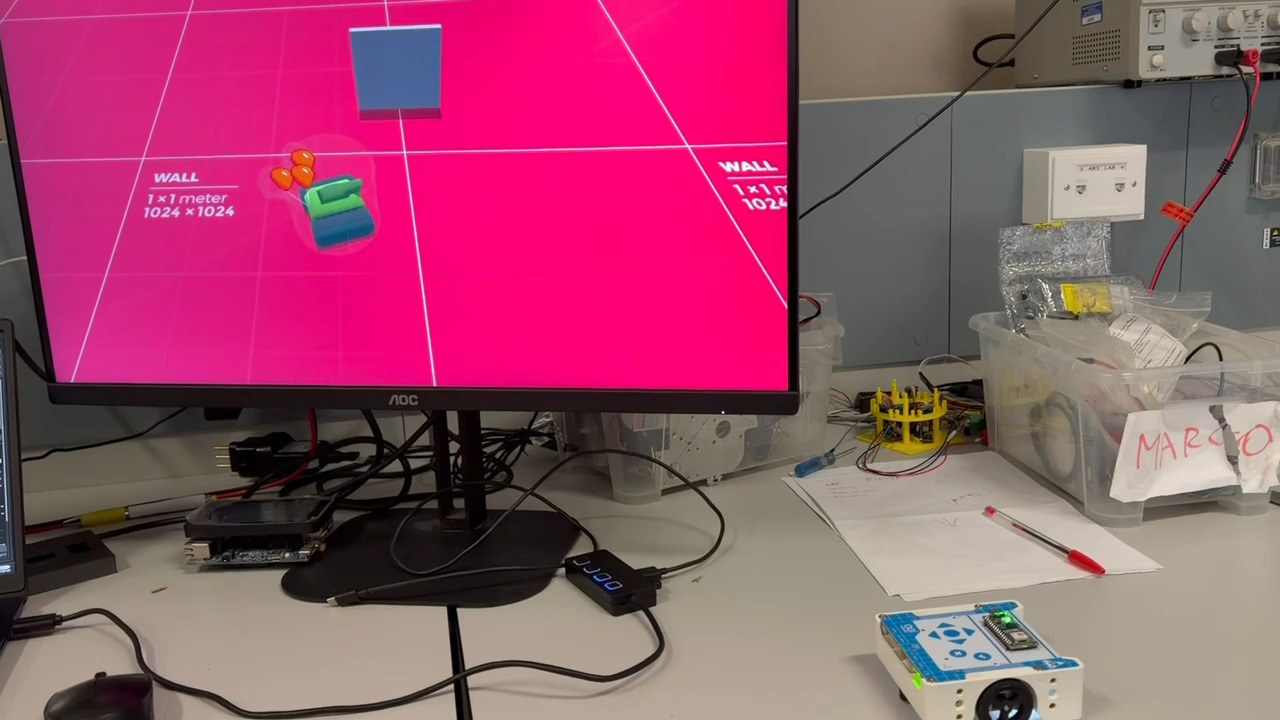
\includegraphics[width=1.0\textwidth]{Images/test-single.jpg}
  \caption{Gemello digitale singolo agente con guida a sterzata.}
  \label{fig:test-single}
\end{figure}
\subsection*{Singolo agente}
Le prime prove sperimentali hanno riguardato il controllo di un singolo gemello digitale. In questa fase l'autore ha costruito famigliarità con l'agente robotico e la cinematica differenziale; sono stati esplorati sistemi di controllo di guida differenti quali un \textit{controllo a sterzata} e un \textit{controllo polare} per la guida del robot. 

Infine, è stato costruito un ambiente virtuale per la navigazione, composto da un piano e un ostacolo, come mostrato in \autoref
{fig:test-single}. In tale ambiente è stato verificato che, qualora il gemello digitale collidesse con un muro e arrestasse il suo moto, di conseguenza anche il gemello reale arrestasse il suo moto.

\begin{figure}[htb]
  \centering
  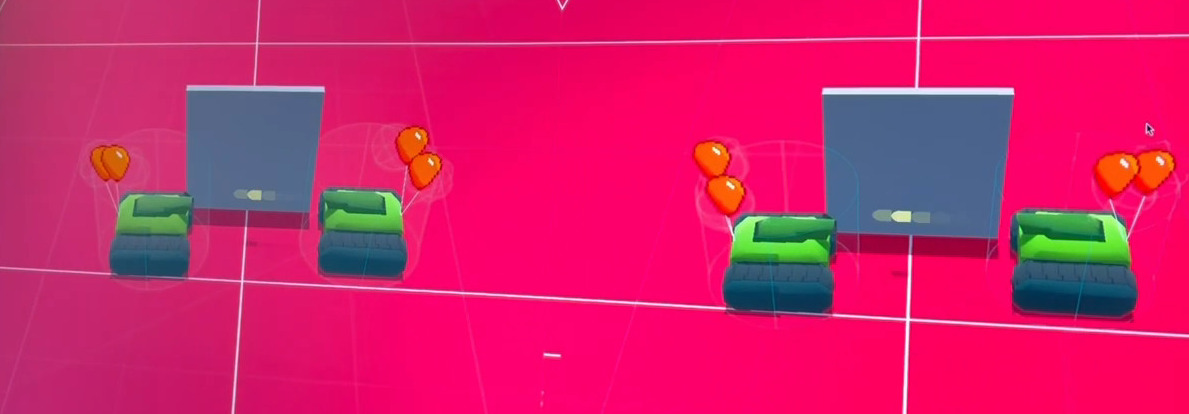
\includegraphics[width=1.0\textwidth]{Images/test-multi.jpg}
  \caption{Due istanze di Godot che espongono l'una all'altra un gemello digitale, implementati anche alcune feature di videogioco.}
  \label{fig:test-multi}
\end{figure}
\subsection*{Multi-agente distribuito}

Concluse le prove singolo-agente, è stata brevemente attestata la capacità del sistema software di gestire più agenti in una singola istanza.

Posto l'obiettivo di rendere distribuito il software, è stato svolto il lavoro necessario affiché sì potessero mettere in comunicazione più istanze di Godot in grado di esporre i gemelli digitali ad essa collegata: in tale fase sono state affrontate e superate con successo le eventuali complicazioni dovuta all'architettura della \textit{MultiplayerAPI}, in particolare la gestione della \textit{authority}, la istanziazione degli agenti remoti e la loro sincronizzazione.

In \autoref{fig:test-multi} sono mostrate due istanze separate di Godot che condividono ambiente virtuale e gemelli digitali.

\subsection*{Multi-agente distribuito e eterogeneo}
\begin{figure}[htb]
  \centering
  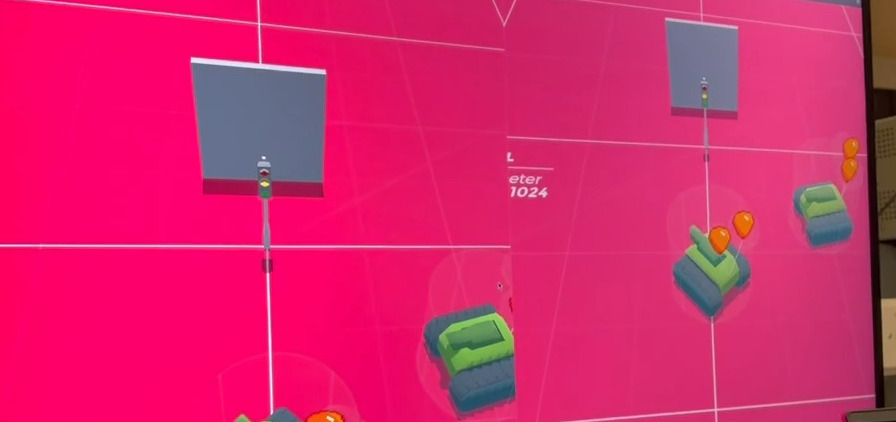
\includegraphics[width=1.0\textwidth]{Images/test-heterogeneous.jpg}
  \caption{Aggiunta di un terzo agente di tipo semaforo.}
  \label{fig:test-heterogeneous}
\end{figure}

Durante la stesura delle fasi conclusive dell'elaborato, è stato osservato che il progetto finale potesse arricchirsi ulteriormente permettendo il collegamento di tipi diversi di gemelli digitali.

Una volta implementata la logica all'interno del sistema, questa è stata corretta da eventuali errori e provata.

Come mostrato in Figura \ref{fig:test-heterogeneous}, è stato implementato un gemello digitale di un oggetto semaforo. Una relativa \textit{Real Agent Interface} è stata prodotta per tale oggetto ed eseguita da una board personalizzata dotata di microcontrollore Arduino Nano ESP32 BLE, il medesimo dell'Arduino Alvik, e di pulsantiera.

\subsection*{Realizzazione di un videogioco digital twin}
Come obiettivo conclusivo del percorso sperimentale, è stato prodotto un prototipo di videogioco di combattimento tra carri armati usando la tecnologia digital twin implementata.

Con l'obiettivo di supportare le dinamiche di gioco sulla infrastruttura realizzata, i gemelli digitali originali degli agenti Alvik sono stati estesi con le seguenti componenti e aggiunte:

\begin{itemize}
	\item È stato implementato un \textbf{sistema di vita} sul gemello digitale del carro. Ogni carro dispone di \textit{tre unità di vita}, raffigurate visivamente da altrettanti \textit{palloncini} legati al retro del carro. Ogni qualvolta il carro riceve un danno perde una unità di vita e un palloncino si scollega e vola via, inoltre: se il carro ha terminato le vite, il carro viene arrestato e viene mostrata visivamente una bandiera bianca a simboleggiarne la resa; altrimenti nel caso avesse ancora vite disponibili otterrà temporaneamente l'invincibilità e non potrà essere colpito da altri giocatori.
	\item A supporto del sistema precedente, è stato implementato un \textbf{sistema di shooting} dotato di tempo di ricarica. È stato prodotto un oggetto \textbf{bullet} (proiettile) e relativo assets, in grado di muoversi lungo un moto parabolico, collidere con oggetti e dotato di tempo di vita e massima distanza. Qualora in bullet interagisca con un carro avvierà le opportune routine di danno.
	\item Un sistema di ripristino è stato implementato affinché lo stato di vita dei carri possa essere ripristinato.
\end{itemize}

Al fine di rendere l'esperienza tanto più coinvolgente possibile, sono stati prodotti assets originali e personalizzati assets pubblici e gratuiti, inoltre è stata realizzata una opportuna arena di gioco. %<- richiama il file "parts/capitolo5.tex" che contiene il primo capitolo
%Si consiglia di creare un nuovo file per ogni capitolo

\chapter*{Conclusione}



\noindent L'implementazione di \textit{Distributed Multi-Agent Digital Twin Environment} prodotta come progetto di tesi offre una vasta gamma di strumenti atti a facilitare lo sviluppo di soluzioni digital twin multi agente con il motore di gioco Godot.

È stato concretamente realizzato il protocollo \textit{Digital Twin Protocol}, fondamenta di tutto il progetto, il quale non solo permette uno scambio bidirezionale semplice e veloce di stato tra i due gemelli, ma anche invocazioni a procedura remota. 
\smallbreak
Al supporto di DTP è stata realizzata una libreria semplice e immediata per la definizione di interfacce \textit{Real Agent Interface} in C++, enfatizzando l'uso di più semplici ma altrettanto sofisticati paradigmi dichiarativi di alto livello, con particolare attenzione alla facilità d'uso e la portabilità per dispositivi embedded e IoT, a cui è seguita una digressione di percorso atta a rendere compatibile la libreria ENet con sistemi embedded basati su ESP32.
\smallbreak
Infine, una suite di componenti e strumenti sono stati realizzati per il motore di gioco Godot, atti alla realizzazione di complessi sistemi multi-agente di gemelli digitali, la quale sfrutta pienamente le API offerte dalla piattaforma per il networking, semplificando drasticamente la realizzazione di sistemi digital twin distribuiti.

I risultati ottenuti soddisfano pienamente gli obiettivi implementativi prefissati, confermando la solidità dell'architettura proposta nell'articolo scientifico su cui si fonda\cite{Russo2025}.
\bigbreak
La conclusione di questo lavoro non è un punto di arrivo definitivo, bensì pone le basi per ulteriori e interessanti sviluppi.

In primo luogo, con l'obiettivo di migliorare la qualità del lavoro svolto finora con il protocollo DTP, si intende introdurre un formato di serializzazione dati binario e leggero, così da ridurre ambiguità e potenziali errori.
\smallbreak
Di notevole interesse per lavori futuri è la ricerca e implementazione di una soluzione peer-to-peer per la comunicazione tra istanze del framework, così da eliminare la corrente soluzione di natura prettamente client-server, e quindi estendere ulteriormente il framework introducendo robusti sistemi ridondanti e distribuiti di gemelli digitali multi agente.
\smallbreak
Infine, sarebbe interessante esplorare la portabilità del framework, o la realizzazione di una sua particolare implementazione compatibile, in grado di eseguire in sistemi embedded.




\addcontentsline{toc}{chapter}{Conclusione} %per fare inserire il capitolo nella tabella dei contenuti
 %<- richiama il file "parts/conclusione.tex" che contiene la conclusione

%Inserisce la bibliografia
\newpage
\addcontentsline{toc}{chapter}{Bibliografia}
\bibliography{bibliography}
\end{document}